\chapter{Results}
\begin{comment}


\end{comment}

\section{Lenard-Jones Potential with direct Summation}
\begin{comment}

\end{comment}

% Plot of the total energy as a function of time

First we look at a simulation with just the lenard-jones-potential. First we have to decide on a good timestep for the simulation. We search for a good $ \mathrm{prefactor} $ for the following equation.
\begin{equation}
	\label{timestepDeterminant}
 \mathrm{timestep} = \mathrm{prefactor} * \sqrt{(m\sigma^2)/\epsilon} 
\end{equation}
To decide on a good timestep a sequence of plots was created as can be seen in Fig. \ref{SimWithTimestep}. 
\par 
As the timesteps gets bigger , the energy in the simulation goes from stable (timestep 0.01) over a drifting behavior (timestep 0.03) to being unstable (timestep 0.05). A good timestep here, would be 0.01 as the simulation is still very accurate and still runs quite fast. 

\begin{figure}
	\begin{center}
		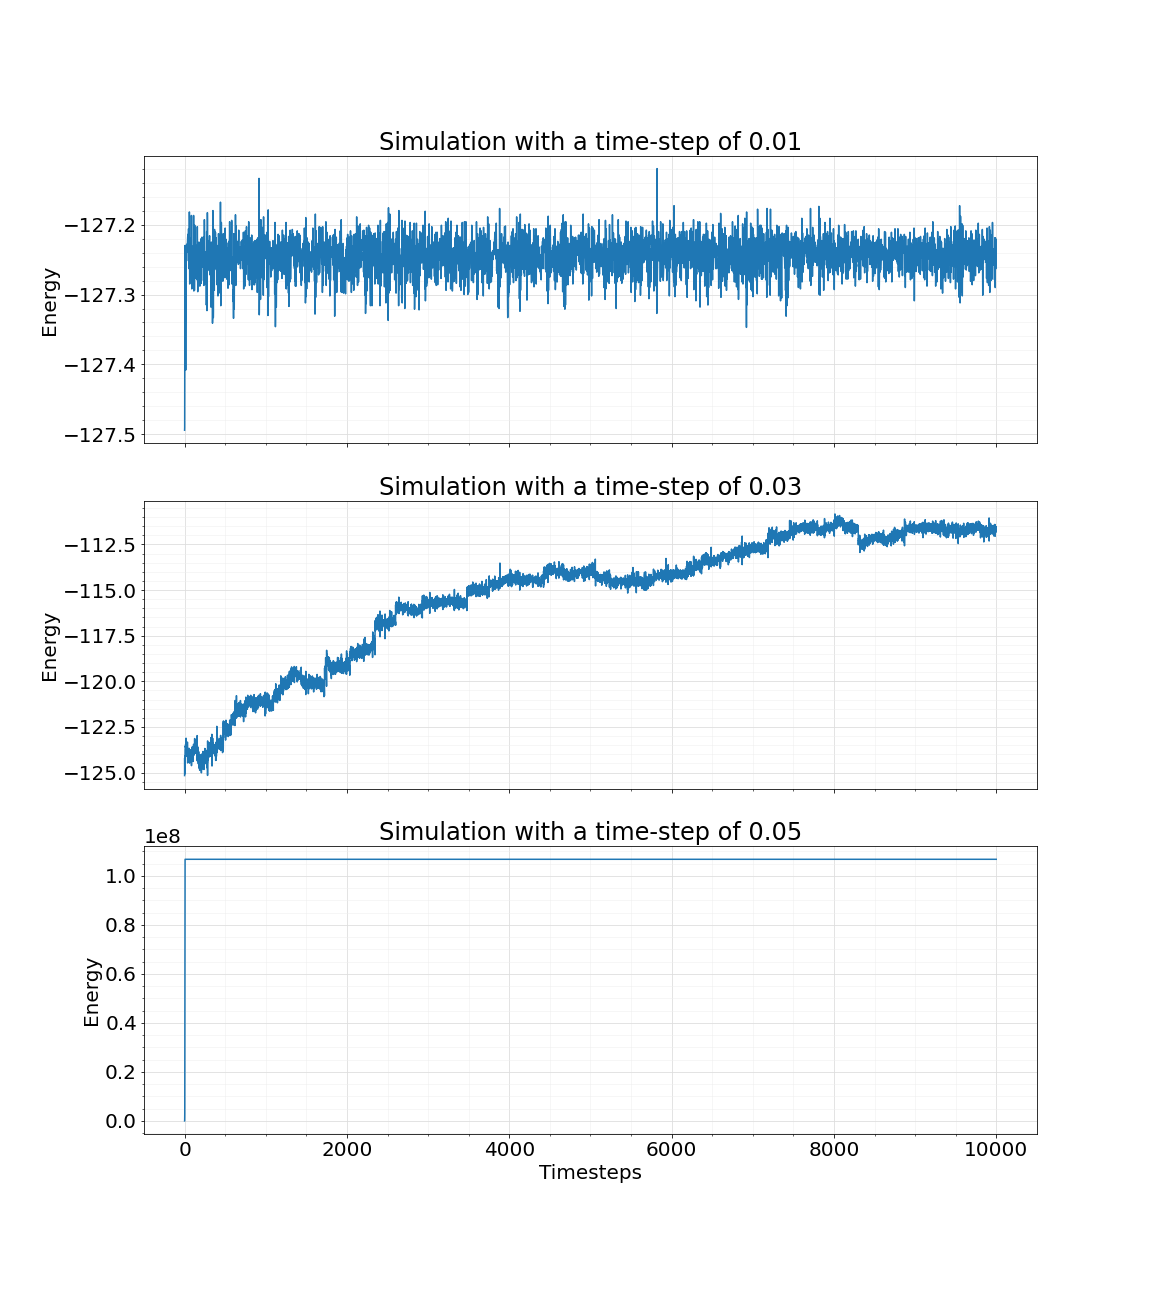
\includegraphics[scale= 1.0]{/home/cm/CLionProjects/MDCode/AData//totalEnergyDrift.png}
	\end{center}
	\caption[Comparison of the energy in the simulation with different timesteps]{Comparison of the energy in the simulation for different timesteps. We run the simulation with $m, \sigma, \epsilon = 1$ for a constant number of steps $n_{steps} = 10000 $}
	\label{SimWithTimestep}
\end{figure}
\par
To visualize the simulation OVITO \cite{ovito} was used and a series of snapshots, visible in Fig. \ref{SimulationSnapshot1} - \ref{SimulationSnapshot3}, was created. The following images show one of the first simulations that was run, where the forces were calculated with the Lenard-Jones-Potential. The simulated cluster has a size of 52 atoms, and was given in the course lecture material \cite{molDymCourse}.
% Simulation Snapshots
\begin{figure}
	\begin{center}
		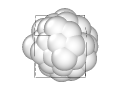
\includegraphics[scale= 0.65]{Figure/1ImageS.png}
	\end{center}
	\caption[Simulation Snapshot 1]{Initial state of the cluster}
	\label{SimulationSnapshot1}
\end{figure}

\begin{figure}
	\begin{center}
		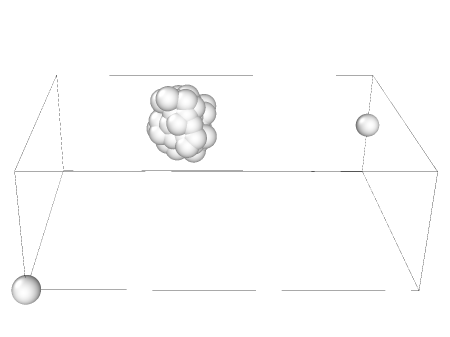
\includegraphics[scale= 0.75]{Figure/2ImageS.png}
	\end{center}
	\caption[Simulation Snapshot 2]{State after 2000 timesteps}
	\label{SimulationSnapshot2}
\end{figure}

\begin{figure}
	\begin{center}
		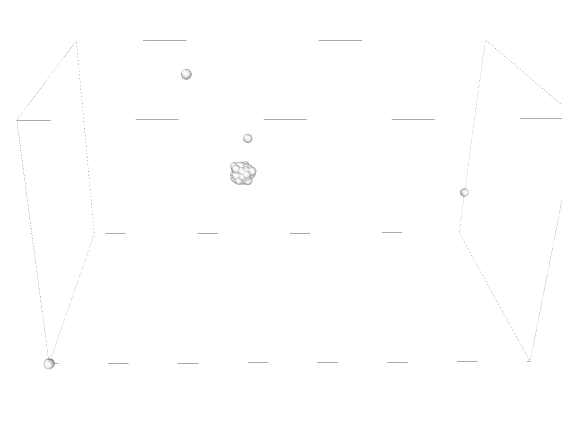
\includegraphics[scale= 0.65]{Figure/3ImageS.png}
	\end{center}
	\caption[Simulation Snapshot 3]{State after 4000 timesteps}
	\label{SimulationSnapshot3}
\end{figure}
As it can be seen in the images \ref{SimulationSnapshot1}, \ref{SimulationSnapshot2} and \ref{SimulationSnapshot3} the Atoms are initially ordered into a cluster, which was given in the course. 
Later in the simulation some of the atoms escaped the initial blob and flew outward separately. 
\section{Simulation with the Berendsen Thermostat}
\begin{comment}
computational complexity 
why on2
optimization not every force is looked at individually as the force resluting form this atom is the same for the other atom but negative
\end{comment}
After incorporating the Berendsen thermostat into the code it is interesting to look at the computational complexity of the simulation. With growing numbers of atoms, the computation-time should grow quadratically. The main culprit for this is the force-computation, as each interaction with all the other atoms in the simulation has to be computed. This is also shown in the next figure as the computation time seems to follow a quadratic function. 
\begin{figure}
	\begin{center}
		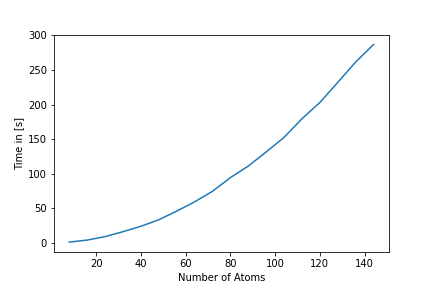
\includegraphics[scale=1]{Figure/plotAtomTimes.png}
	\end{center}
	\caption[Comparison of the time needed to simulate 8 to 192 Atoms]{Comparison of the time needed to simulate 8 to 192 Atoms. The simulation was run with the parameters $\sigma, \epsilon = 1$ , $m = 12\mathrm{u}$ for a total of 10000 steps with a duration of $\mathrm{timestep} = 0.01\sqrt{(m\sigma^2)/\epsilon} $. The relaxationtime of the thermostat was set to 50 $\mathrm{timestep} $, which is very low, but was done to get the simulation stable in all cases. The thermostat had a target-temperature of 275K.} 
	\label{PlotSimulationTimeBerendsenThermostat}
\end{figure}
Although all the interaction between all the atoms are computed, the individual forces do not carry the same weight to the force that affects the atom. It should be rather clear that, the further apart atoms are, the smaller the forces get. After a certain distance it gets so small that it can be ignored. This leads to the idea to use neighborhood-lists that ignore the atoms outside of a certain radius, which has been done in the next section.

\section{Simulation with the Neighborhood-List}
\begin{comment}

\end{comment}
After running the simulation in the previous section, it was clear that they follow a computational complexity of the order O(N²). This can be reduced to a linear order O(N) with the usage of neighborhood-lists. Only the atoms in a certain radius around the atom will be considered and a force will be added to the total force affecting the atom. This can be seen in Fig. \ref{PlotSimulationTimesCutoffNew}.
\begin{figure}
	\begin{center}
		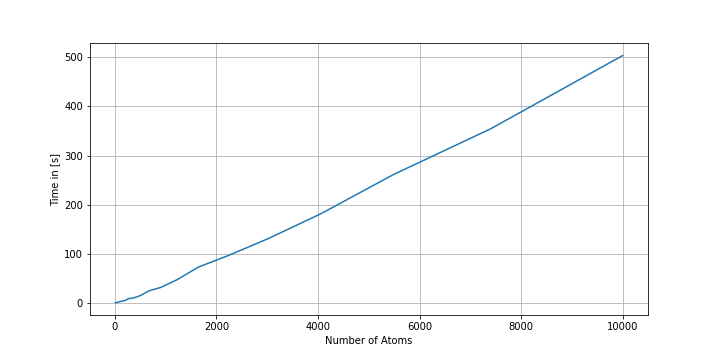
\includegraphics[scale=1.25]{Figure/plotAtomTimesMoreData.png}
	\end{center}
	\caption[Comparison of the simulationtime with neighborhood-lists ]{Comparison of the simulationtime with Neighborhood-lists. Basic parameters are the same as in Fig. \ref{PlotSimulationTimeBerendsenThermostat}, but with an additional cutoff of 2.5$\sigma$}
	\label{PlotSimulationTimesCutoffNew}
\end{figure}

\section{Simulation with the Embedded-Atom Method Potential}
\begin{comment}
1 graph
- potential energy gets less with an increase to the clustersize
- the 

2 
Heat capacity and latent heat should converge
\end{comment}
In the next step the embedded-atom method potential was used to compute the potential energy and the forces between the atoms. A neighborhood-list was also used. With this it is possible to look at the actual physical properties of the materials - in this case gold. 
\par 
\begin{figure}
	%Higher than 9 just nicer to look at!!!
	\begin{center} 
		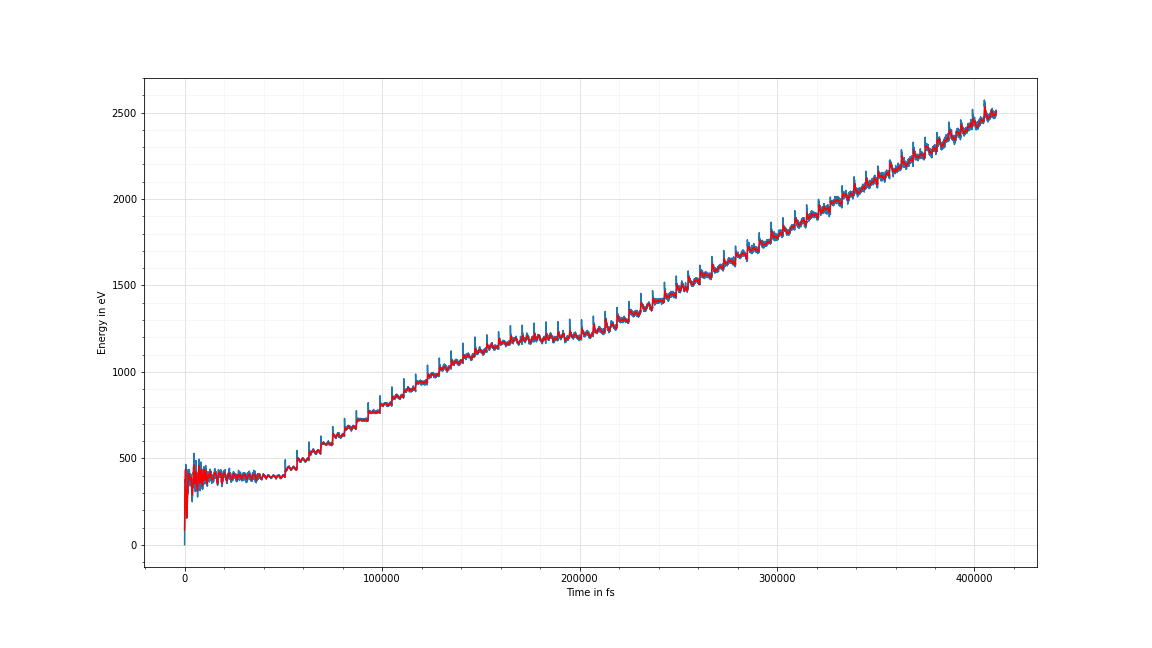
\includegraphics[scale=1.15]{/home/cm/CLionProjects/MDCode/AData/Clusters/kineticEnergyCurve14.png} 
	\end{center} 
	\caption[Gold cluster simulation: Kinetic Energy vs Time]{Gold cluster simulation: Kinetic Energy vs Time} 
	\label{GoldClusterSimulationKinVsTime} 
\end{figure} 


\par 
In Fig.  \ref{GoldClusterSimulationTemperaturEnergy4In1} energy and temperature for different cluster sizes are plotted. It is possible to extract the melting point, the heat-capacity and the latent-heat from this diagram. This can be seen in the next Fig. \ref{GoldClusterSimulationVsClustersize} in relation to the size of the atom-cluster.
\par 
The first interesting property is the melting point of the cluster, which can be seen in the different curvatures in the graphs in figure \ref{GoldClusterSimulationTemperaturEnergy4In1} (for the red graph at 900K for example). The melting point increases as the clusters get bigger, but is still not not near it's macroscopic equivalent of 1337K. 
%TODO no real source read out of a table from school lol
\par
It can also be seen that the potential energy of the average atom decreases with bigger clustersizes. To explain this, the ratio of surface to volume of the cluster and the fact that atoms at the border of the cluster need to have a higher energy, have to be considered. With increased clustersizes a smaller percentage of atoms is at the edge which leads to an increases in the total energy of the cluster. 
The slope of the jump at the melting point also increases with bigger clustersizes. For many atoms these curves would be piecewise linear with a high-slope section around the melting point. The simulated system seems to converge to that. 

\begin{figure}
	\begin{center} 
		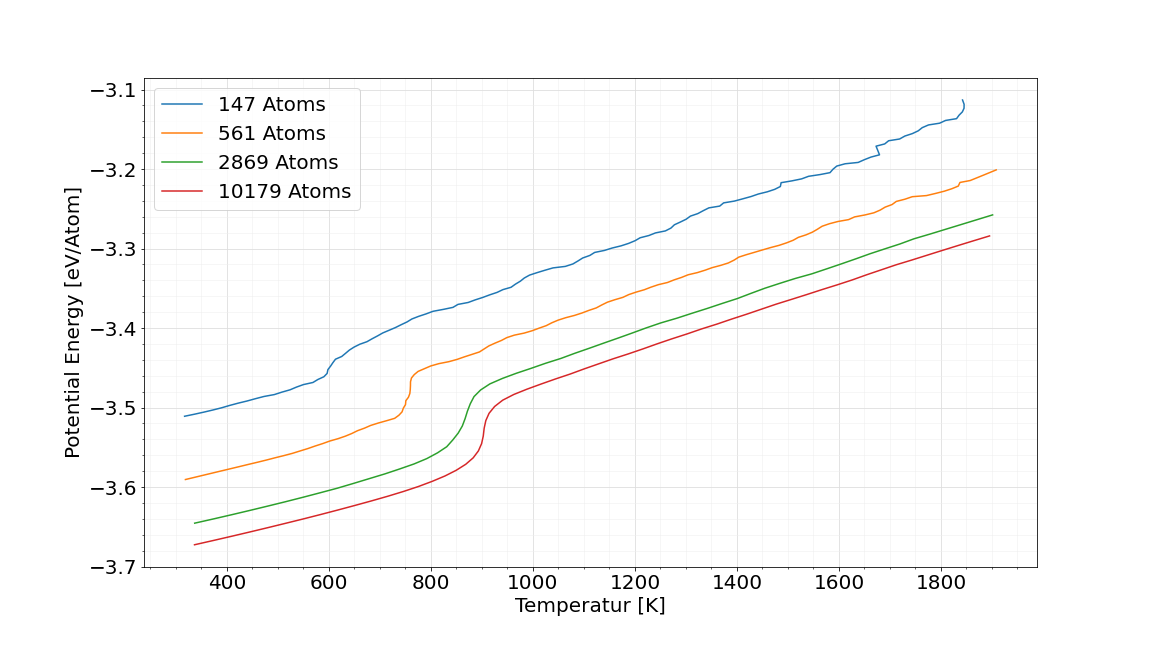
\includegraphics[scale=1.15]{/home/cm/CLionProjects/MDCode/AData/Clusters/temperaturPotentialEnergyCurveMoreInOne.png} 
	\end{center} 
	\caption[Gold cluster simulation]{Gold cluster simulation with different quantities of atoms} 
	\label{GoldClusterSimulationTemperaturEnergy4In1} 
\end{figure} 

In the diagram of Fig. \ref{GoldClusterSimulationVsClustersize} which plots the heat capacity and the latent heat, it can be seen that both seem to converge. On the other hand, the melting point still seems to increase as it is still away from it's true melting point.

\begin{figure}
	\begin{center} 
		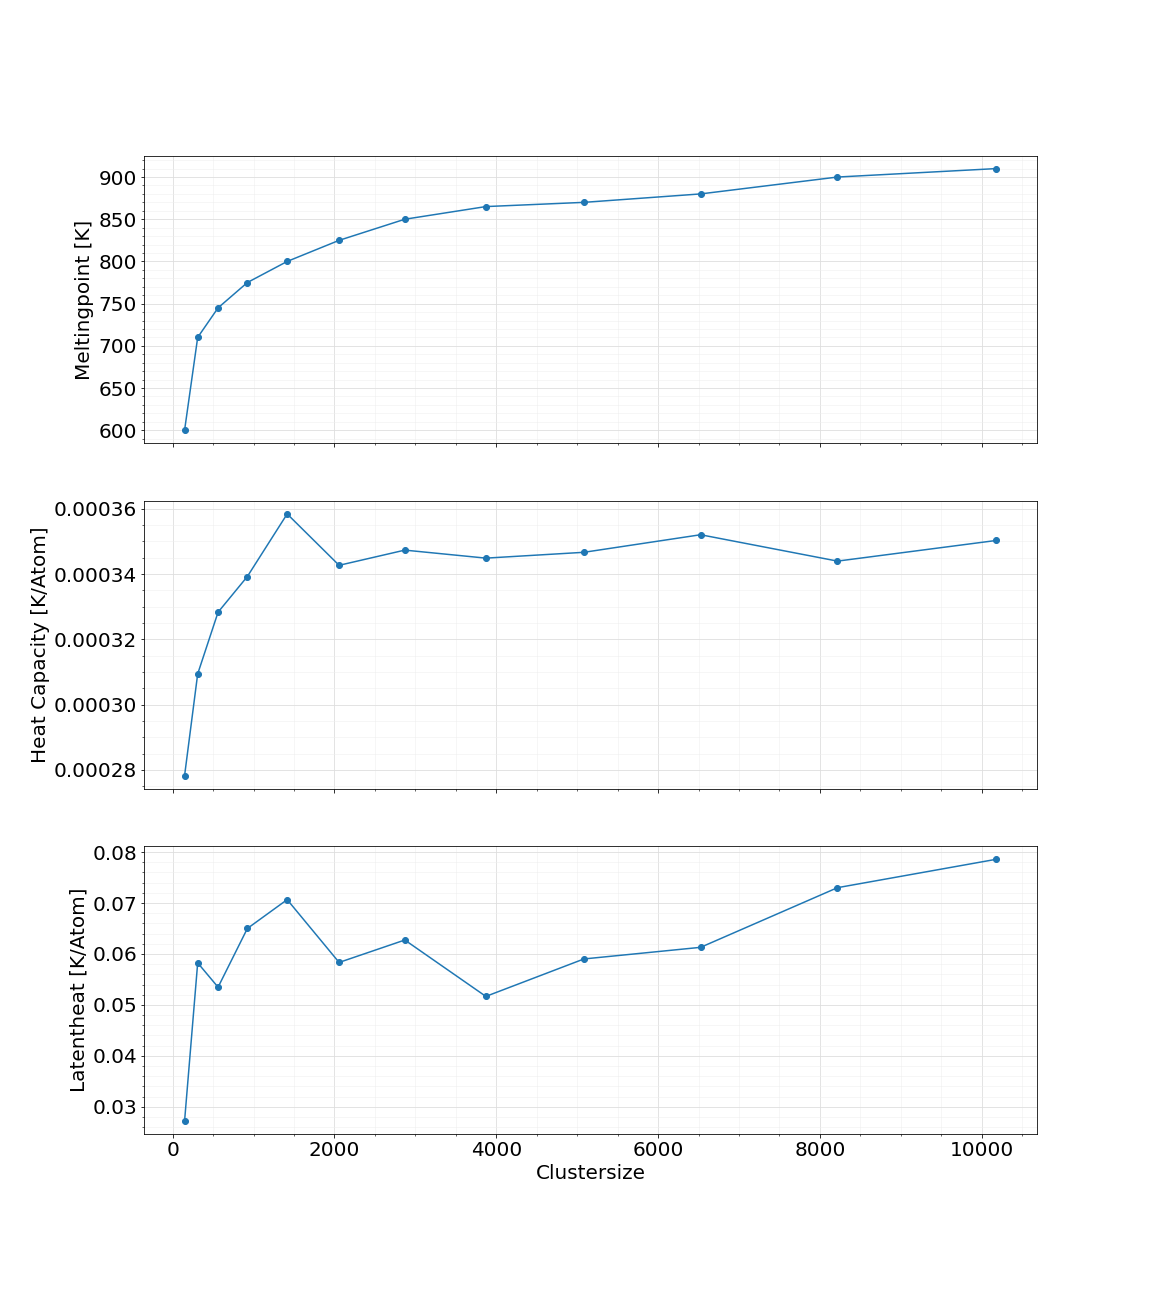
\includegraphics[scale=1.15]{/home/cm/CLionProjects/MDCode/AData/Clusters/VsClusterSizeAll.png} 
	\end{center} 
	\caption[Melting point, heat capacity and latent heat vs clustersize]{Melting point, heat capacity and latent heat vs clustersize} 
	\label{GoldClusterSimulationVsClustersize} 
\end{figure} 
